%!TEX root = thesis.tex

\chapter{The Spatio-Temporal Topic Model} \label{ch:topic-models-detail}

\section{Topic Models and Latent Dirichlet Allocation}

% KL-Divergence is a measure of the information lost when approximating one distribution with another, equal 0 if the distributions are identical and $\infty$ if they do not have the same support. If we sample a taxon randomly from the estimated distribution, and that taxon has probabilities $p,~q$ under the estimated and true distributions respectively, the KL-Divergence gives the expected value of $log \frac{p}{q}$.

%%%%%%%%%%%%%%%%%%%%%%%%%%%%%%
%%% What is a topic model? %%%
%%%%%%%%%%%%%%%%%%%%%%%%%%%%%%
Topic models are a family of probabilistic latent variable model, developed as a tool for document and word classification according to semantic clusters called `topics'. Topic models aim to find word clusters derived solely from word co-occurrence, and are thus suitable for large, unlabelled datasets. For instance, in a corpus of of news articles, a successful topic model might learn that the words `film', `show', `audience', and `actor' form one cluster, and `budget', `market', `plan', and `spending' form another. These natural groupings of words give topic models their name.

Compared to other unsupervised learning methods, a document is treated directly as a collection of many of discrete-valued variables (words), rather than as a single high-dimensional vector. As a result, topic models provide a much more direct way to reason about and place priors on individual observations, ultimately leading to powerful, interpretable representations of document collection datasets.

Topic models posit a generative model for text documents: $K$ topics are defined, each formulated as a probability distribution over words from a finite vocabulary of size $V$. Each document is defined by a distribution of topics and a total number of words. The process for generating a document is modelled such that, for each word, first a topic $z$ is drawn from the topic distribution for its document (the document-topic prior $\theta_d$). Then, a word $w$ is drawn from the corresponding topic (the topic-word distribution $\phi_{z}$). The computational goal of topic modelling algorithms is to invert this process, observing the words from a set of documents and inferring the posterior over topic assignments $p(\boldsymbol{z} | \boldsymbol{w})$. In addition to the maximum likelihood topic assignments for individual words, this posterior also gives access to the document-topic prior matrix $\Theta$ and global topic-word distribution matrix $\Phi$. Topic models were first proposed with identical, uniform document-topic priors under the name Latent Class Analysis (LCA) \citep{Hofmann2000}, and subsequently with independent document-topic priors as Probabilistic Latent Semantic Analysis (PLSA) \citep{Hofmann2001} in the early 2000s, followed throughout the decade by many more variants where slight modifications to the generative model have been proposed \citep{Blei2010}.
\todo[inline]{I think it would be appropriate to make the connection to the large and even earlier literature on multi-dimensional scaling (which includes PCA and many other linear and non-liner methods) which is arguably a form of topic modeling, but unarguably a close conceptual relative. Draw from Blei 2003}
Although PLSA is extremely general, with no further assumptions topic models are unlikely to find intuitive topics and also often generalize poorly as they are prone to overfitting \citep{Blei2003}.
Latent Dirichlet Allocation improves this situation, while minimally decreasing the expressive power of the model in practice by making a further assumption, namely, placing independent Dirichlet priors on each individual document topic prior $\theta_d$ and topic word distribution $\phi_z$.
Recall that the Dirichlet distribution $Dir(\theta; \boldsymbol{\alpha})$ is the multivariate generalization of the Beta distribution, i.e. a distribution over the $K-1$ dimensional simplex with parameter $\boldsymbol{\alpha} \in \mathbb{R}^K$. In other words, it is a distribution over the $K$ dimensional discrete-valued probability mass functions (PMFs). To be exact the, Dirichlet distribution is a (conjugate) prior for categorical and multinomial distributions, with probability density function (PDF):
\begin{equation}
P(\theta|\boldsymbol{\alpha}) = \frac{\Gamma(\sum_{i=1}^{K} \boldsymbol{\alpha}_i)}{\prod_{i=1}^{K} \Gamma(\boldsymbol{\alpha}_i)} \prod_{i=1}^{K} \theta_i^{\boldsymbol{\alpha}_i -1}
\end{equation}
Where $\Gamma$ denotes the gamma function.

\begin{figure}
	\centering
	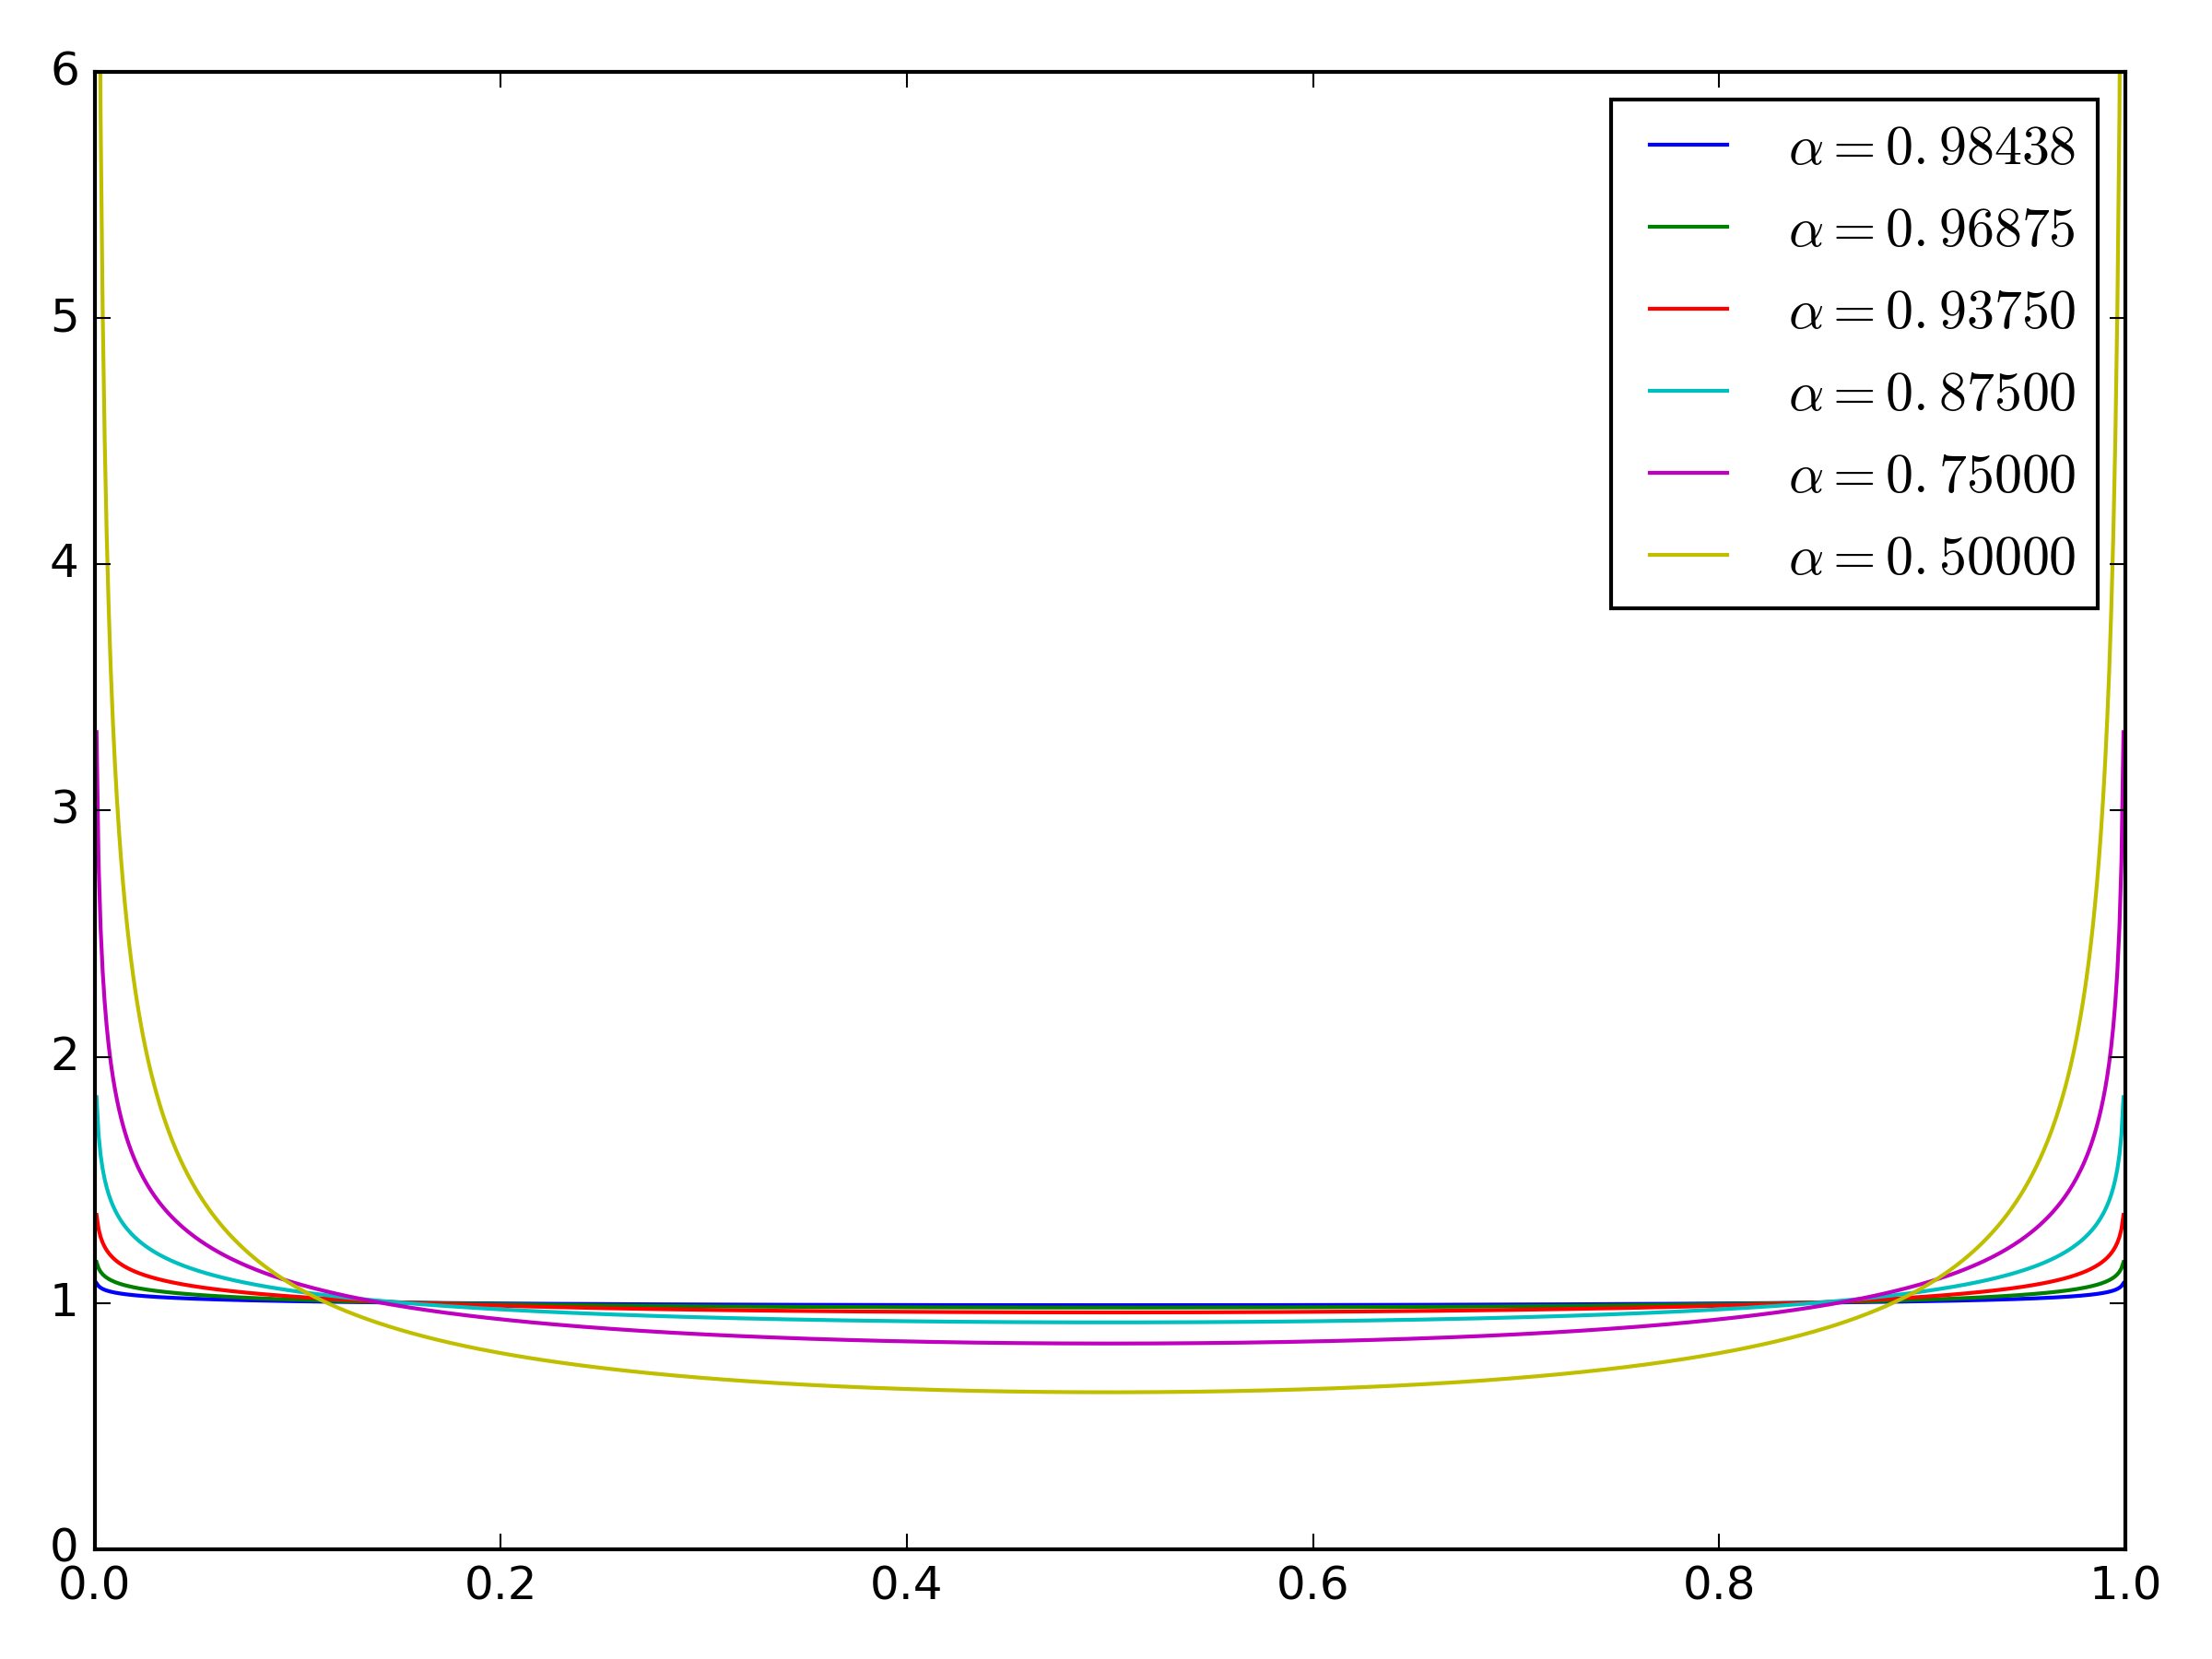
\includegraphics[width=0.65\columnwidth]{figures/beta.png}
	\caption{
		PDFs of Dirichlet distributions with 2D symmetric parameters $\alpha$. These can be used as a prior over the 2D PMFs. Note that this means there is $K-1 = 1$ degree of freedom, i.e. this is a prior for a Bernoulli random variable and this case is identical to a $\mathrm{Beta}(\alpha_0, \alpha_1)$ distribution. It is helpful imagine each of these curves as giving a distribution of probabilities for coins from an unfair coin factory, where the average over all coins looks fair, but (for large $\alpha \approx 0$) most individual coins are very unfair. For a K-dimensional Dirichlet distributions, the corresponding analogy is a prior for unfair K-sided dice.
	}
	\label{fig:beta-pdf}

\end{figure}

% \todo[inline]{What is gamma? What does alpha mean?  These "obvious" things should be as explicit as possible.}

It has mean $\boldsymbol{\alpha}_i / \sum_i \boldsymbol{\alpha}_i$ and when $\sum_i \boldsymbol{\alpha}_i < 1$ is said to be `sparse', meaning the pdf has most of its mass on the corners of the simplex, and typical samples have few non-zero entries. In the case of LDA, a symmetric Dirichlet prior is chosen, where $\boldsymbol{\alpha}_i = \boldsymbol{\alpha}_j ~~\forall i, j$, and the concentration, $\alpha = \sum_i \boldsymbol{\alpha}_i$, is considered as a hyperparameter. Fig.~\ref{fig:beta-pdf} illustrates the effect of varying $\alpha$. Choosing a symmetric, sparse Dirichlet prior for the topic-word distribution encodes the assumption that few words are strongly associated with a topic, some words are weakly associated with a topic, and most words are not at all associated with a topic without requiring any external information about which individual words are associated with which topics.

The posterior for $\theta$ given observations $z_i \sim Cat(\theta),~i = 1, \ldots n$ can be easily derived using Bayes' rule to be $P(\theta | \boldsymbol{N}) = Dir(\alpha + \boldsymbol{N})$, where $\boldsymbol{N}$ is the vector of counts for each of the $K$ possible values of $z$, and consequently the predictive distribution for $z_{n+1}$ is given by \citep{BishopCh2}:
\begin{equation}
\begin{split}
P(z_{n+1}=k | \alpha, \boldsymbol{z}) =& \int P(z_{n+1}=k | \theta) P(\theta | \alpha, \boldsymbol{z}) d\theta\\
=& \int \theta_k Dir(\alpha + \boldsymbol{N}) d\theta\\
=& \frac{N_k + \alpha}{\sum_{j=1}^K N_j + \alpha}
\end{split}
\end{equation}

Although exact inference of the full LDA posterior $P(\boldsymbol{z} | \boldsymbol{w})$ is intractable, the posterior for a single topic assignment $z_i$ can be estimated with a collapsed Gibbs sampler based on a the product of the predictive distributions due to $\theta$ and $\phi$ \citep{griffiths2004}. Given a set of observed words $\textbf{w}$, and topic assignments for all words except the current word, $w_i$, $\boldsymbol{z_{-i}}$ with counts $N^v_k$ being the number of times word $v$ was assigned topic $k$ and $N^k_d$ the number of times topic assignment $k$ has been used in document $d$
\begin{equation} \label{eqn:posterior}
P(z_i = k | \boldsymbol{z_{-i}}, \boldsymbol{w}) \propto \left(\frac{N^k_d + \alpha}{\sum_{j=1}^K N^j_d + \alpha}\right)
   \left( \frac{N^{w_i}_k + \beta}{\sum_{v=1}^V N^v_k + \beta} \right)
\end{equation}

Various other methods for approximate posterior inference for LDA have been explored, particularly variational methods and more recently stochastic gradient approximations to variational methods (For a comprehensive review, see \citep{geigle2016}). Despite the efficiency of these methods, they lack the appealing anytime,
(in the sense of Zilbertstine, \citep{zilberstein1996anytime})
% \todo[inline]{maybe say "anytime (in the sense of Zilberstein)"}
online aspect of a sampling based approach, and are much less flexible to modification of the model. For these reasons in this work we rely only on the Gibbs sampling based approach.

\section{Realtime Online Spatio-Temporal Topic Models}
\begin{figure}
\begin{center}

\subfloat[]{
\hspace{1.2cm}
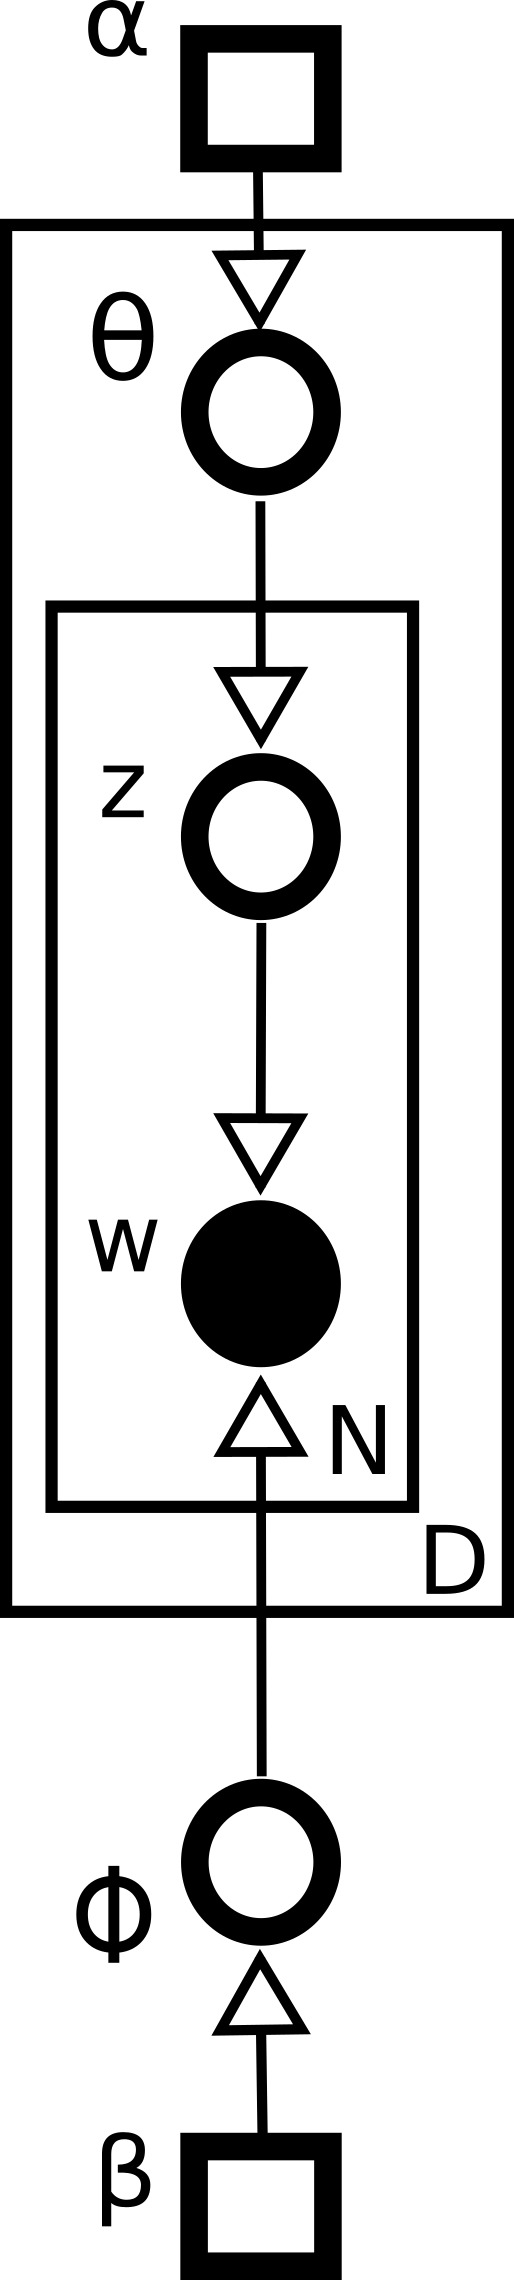
\includegraphics[width=0.13\columnwidth]{figures/lda_pgm.png}
\label{fig:lda-pgm}
} \hfill
\subfloat[]{
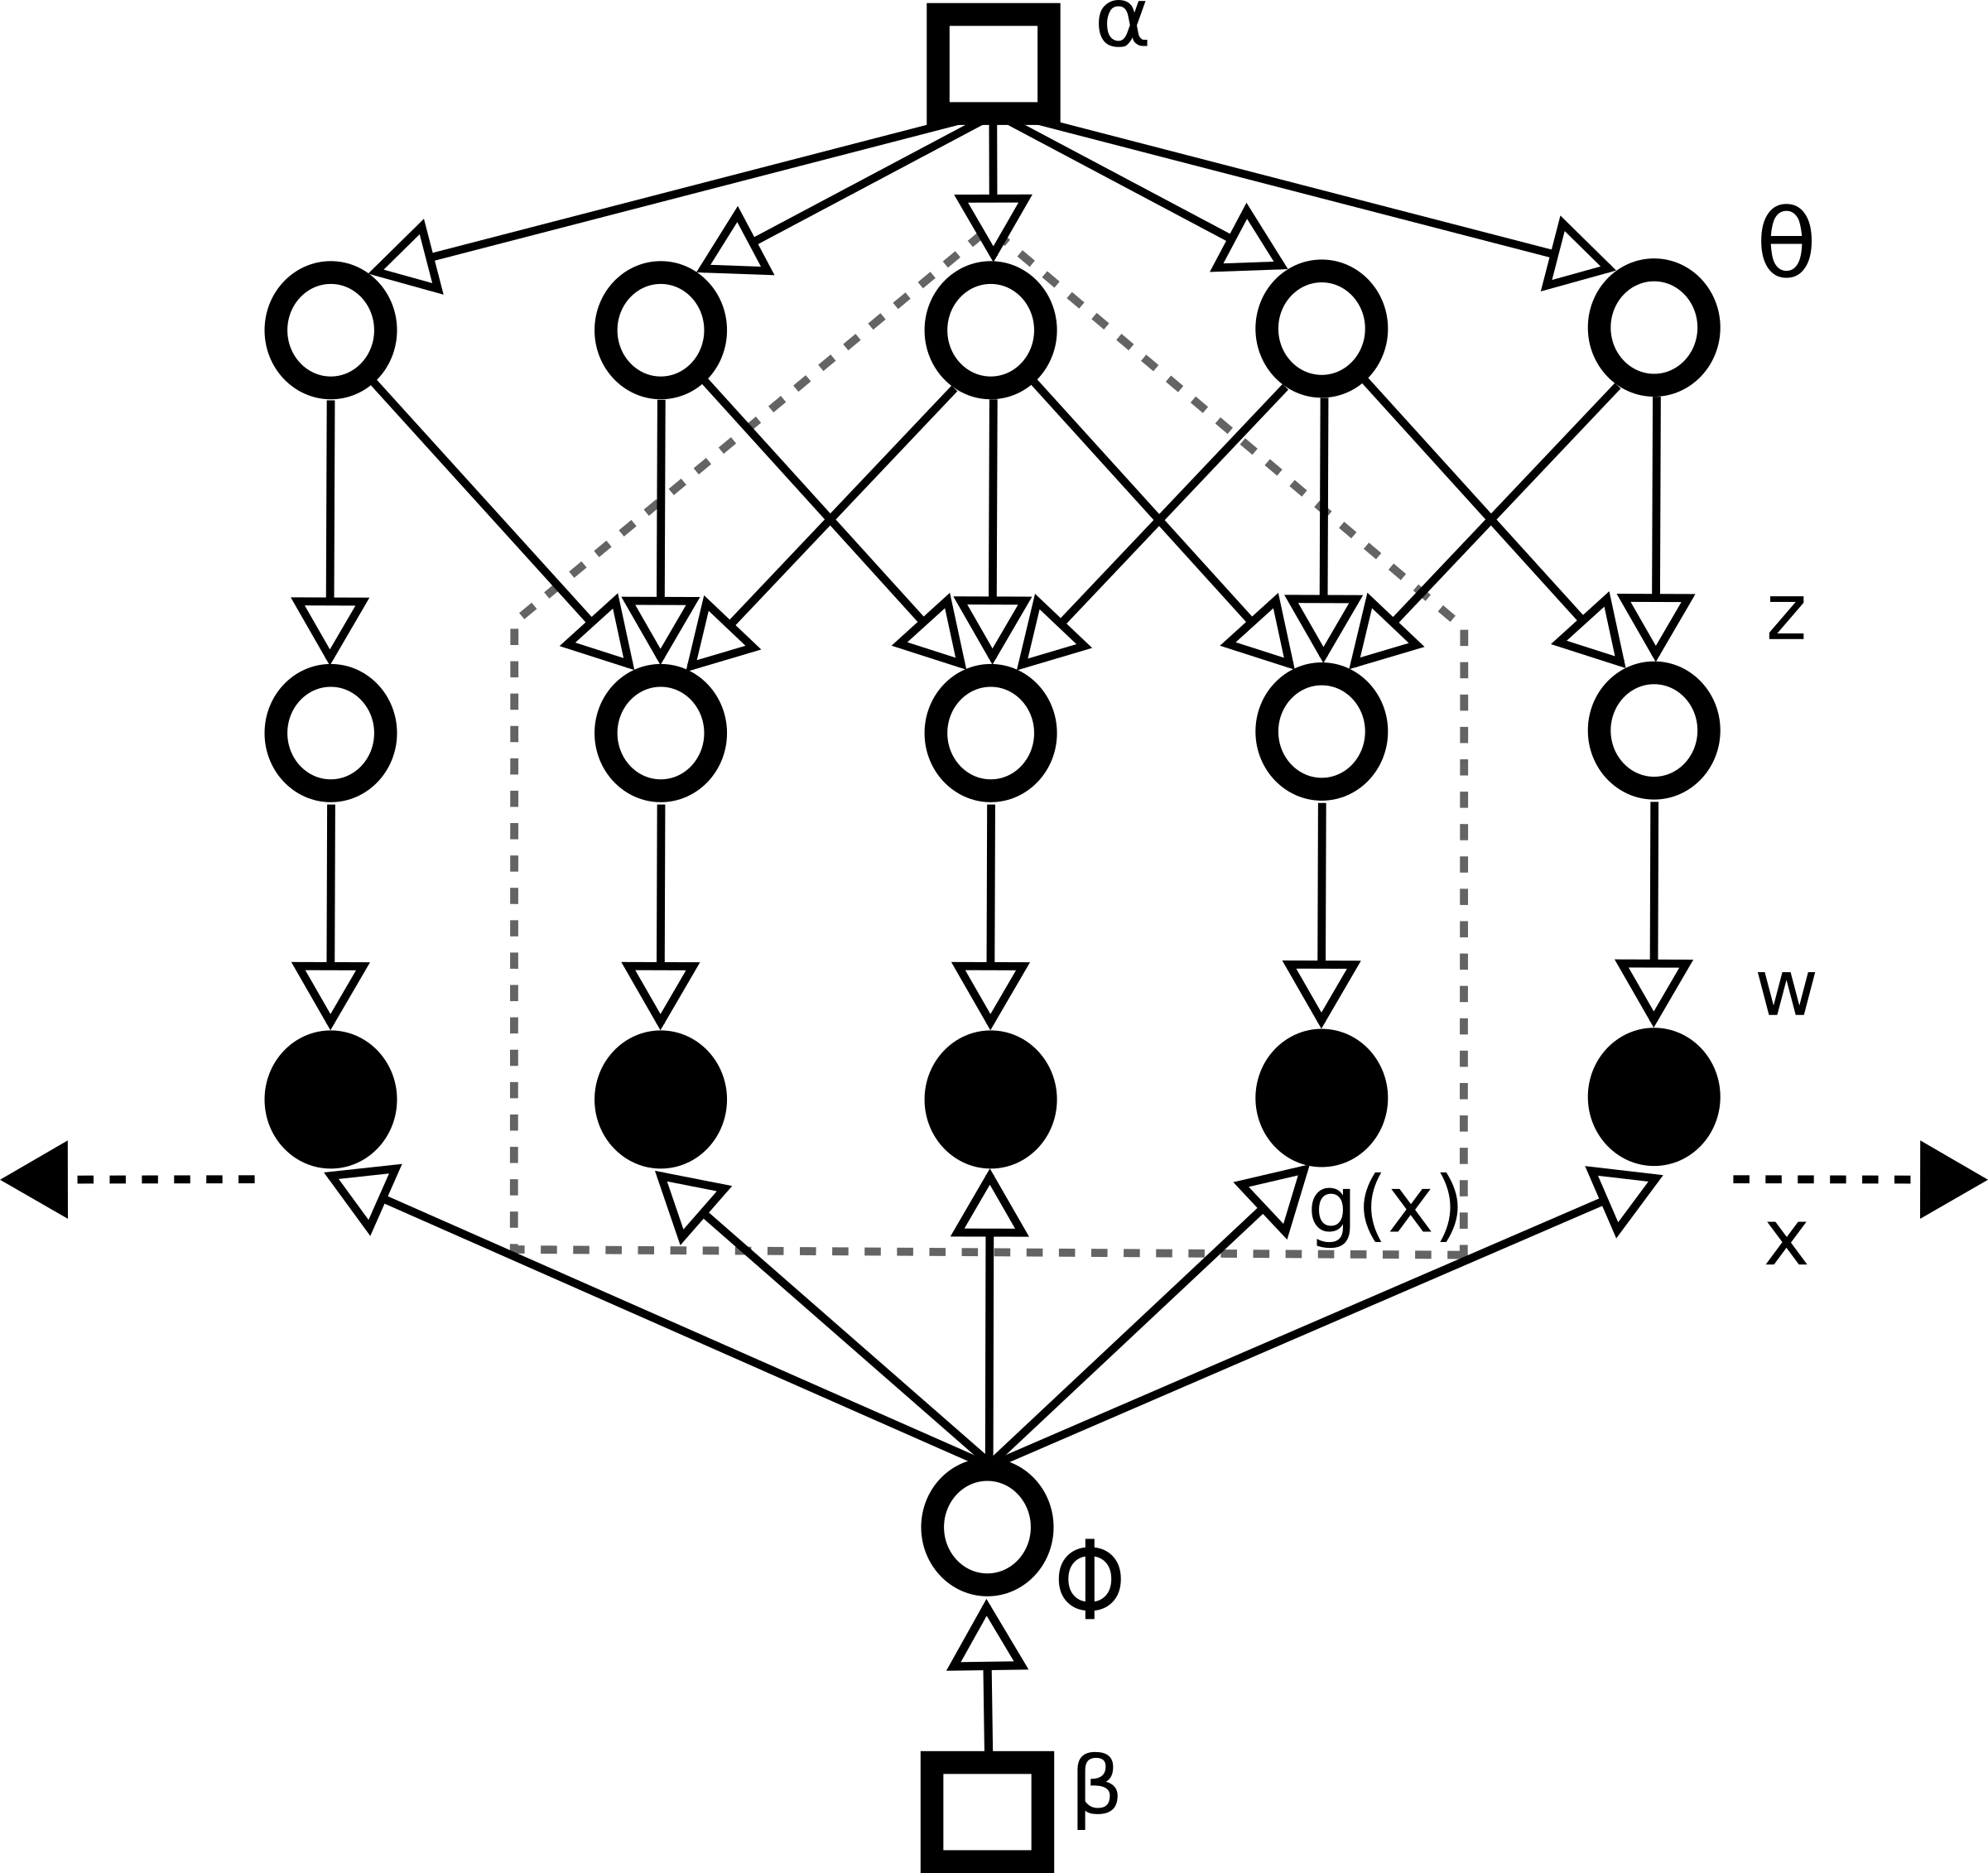
\includegraphics[width=0.6\columnwidth]{figures/rost_pgm.png}
\label{fig:rost-pgm}
}
\end{center}

\caption{
	\emph{Graphical models for topic models:}
	\protect\subref{fig:lda-pgm} Graphical model for Latent Dirichlet Allocation. Words within a document are conditionally independent given their topic assignments $z$ and the topics $\phi$, which in turn are conditionally independent given the topic prior $\theta$ for the associated document.
	\protect\subref{fig:rost-pgm} The graphical model for spatio-temporal topic models relaxes these independence assumptions, as the topic prior is shared by all topic assignments within overlapping spatio-temporal neighborhoods (represented by the dashed pentagon).
}
\label{fig:pgms}
\end{figure}

%%%%%%%%%%%%%%%%%%%%%%%%%%%%%%%%%%%%%%%%%%%%
%%% How has this been used for non-text? %%%
%%%%%%%%%%%%%%%%%%%%%%%%%%%%%%%%%%%%%%%%%%%%
Although LDA has been developed and used primarily in the context of modelling collections of text documents, its fundamental assumptions are compatible with an extremely wide range of applications. Virtually any feature function may be quantized or otherwise tweaked to produce discrete-valued pseudo `words' and collected into `documents'. Sparse, probabilistic `topics' are an attractive, interpretable form of dimensionality reduction for wide variety of domains. Non-textual descendents of LDA have most extensively been used in computer vision applications such as learning natural scene categories \citep{FeiFei2005}, taxonomies of images \citep{bart2011}, human action categories from video \citep{Niebles2008}, and image-caption pairing \citep{Blei2003Captions}. Further works illustrate how LDA can be used in bioinformatics, such as for learning genealogies (taxonomies of species) based on their collections of gene sequences \citep{Pritchard2000}. 

This body of literature hints that the LDA family of models is very general, and could be considered for a much broader set of applications where unsupervised representation learning is desired. One of the aims of this thesis is to demonstrate the breadth of this set. To clearly enumerate assumptions which must be met by an LDA application: (1) The data must be comprised of collections of discrete observations, (2) the observations within a collection must be conditionally independent given a set of topics and a prior over these topics, (3) the observations in separate collections must be conditionally independent given the topics and a symmetric Dirichlet prior, and (4) the topics must be conditionally independent given another symmetric Dirichlet prior.

%%%%%%%%%%%%%%%%%%%%%%%%%%%%%%
%%% What does ROST add? %%%
%%%%%%%%%%%%%%%%%%%%%%%%%%%%%%
Nevertheless, real-world data rarely meet these criteria exactly. In particular, observations associated with a particular place or time cannot usually be considered independent from nearby observations (Assumption 3). While we could accommodate this by simply increasing the size of our collections of observations, this choice would come at the cost of decreasing the spatio-temporal resolution of the learned document-topic priors. What we would like is to enforce smoothness rather than equality between nearby topic priors.

The Realtime Online Spatio-temporal Topic model ROST, implements exactly such a variant of Latent Dirichlet Allocation \citep{Girdhar2014}. With ROST, fully discrete \emph{documents} are replaced by \emph{neighborhoods}, each comprised of a topic prior and a collection of observations. We denote the neighborhood of a spatial, temporal or spatio-temporal location $x$ by $g(x)$. Crucially, neighborhoods may be overlapping, and consequently the priors for nearby neighborhoods are not independent -- instead they must describe an intersecting set of observations (see Fig.~\ref{fig:pgms}).

Formally, ROST includes the same 3 hyperparameters as LDA, namely $\alpha$, the Dirichlet prior concentration on each $\phi_z$, $\beta$, the Dirichlet prior concentration on $\theta_{g(x)}$ (with the neighborhood at $x$ replacing the document index $d$), $K$, the number of topics, as well as an additional hyperparameter, $g$, the spatio-temporal extent of a neighborhood. Increasing $g$ yields larger neighborhoods, where individual topic priors must account for more varied observations, are more overlapping with their neighbors, and therefore learning gives smoother document-topic distributions. Conversely, as $g$ decreases to 0, ROST becomes identical to LDA and the local topic priors have no tendency towards spatio-temporal smoothness. To implement posterior inference with the collapsed Gibbs sampler, the only change required to Eqn.~\ref{eqn:posterior} is to replace the document $d$ with the neighborhood $g(x)$ if word $w_i$ was observed at location $x$.
% \todo[inline]{Mention the kernel and $g_\sigma$?}
% \todo[inline]{Nice, but not critical as this is review and is getting long, but it would a nice exposition. --gd}

The authors have shown that the spatio-temporal smoothness assumption leads to more semantically relevant topics, in real-time computer vision problems as well as other domains \citep{Girdhar2012, Girdhar2014a, Girdhar2016}. The combination of smoothness and sparcity assumptions consistently leads the map of $\theta_x$ to contain regions with high probability of a single topic, with somewhat less-sparse boundaries between them. Because these assumptions are implemented as priors, precise knowledge of `how smooth' and `how sparse' is not required, in contrast to a harder or non-Bayesian approach. As a result, ROST produces remarkably natural, interpretable topic maps for a wide variety of datasets without an onerous hyperparameter tuning procedure.

\section{Topic Models in Practice} \label{sec:topic-models-inpractice}
Although topic models are a relatively robust modelling technique, recovering semantically meaningful topics still requires careful problem setup. This part of the process is often downplayed in the literature as less-than-generalizeable, nevertheless it is important to obtaining the desired data representation. The applications outlined in this thesis at least partially aim at exploring some of these issues, and how they can be systematized for varied applications and application domains.

%%%%%%%%%%%%%%%%%%%%%%%%%%%%%%%%
%%% Massaging the features   %%%
%%%%%%%%%%%%%%%%%%%%%%%%%%%%%%%%
The first issue encountered by an aspiring topic-modeller is how to obtain features which meet the assumptions of the model. Even in the text-modelling literature, where discrete-valued observations (words) and collections (documents) are readily available, significant pre-processing is common, including removing stop words and rare words, as well as stemming. These steps ensure a bag-of-words model is appropriate, ensuring that all the data is relevant to a semantic interpretation in addition to minimizing the importance of structure not captured by a histogram of words. These measures also have significant beneficial side-effects: stop words often comprise a significant portion of the dataset, so removing them significantly increases the variability between document-word distributions while greatly decreasing the total number of topic assignments to learn. In addition, stemming can greatly reduce the vocabulary, reducing the dimensionality of each word-topic distribution. In the context of natural language processing, these measures are acceptable -- the set of stop words in English is relatively small and can be easily listed, and reasonably performant stemming models are available.

Nevertheless, often the most difficult step in setting up a topic model is formulating a feature function with similar properties. In offline contexts, for a given feature function, filtering the most common and least common words is often a reasonable heuristic approximating removing stop words to enhance the variability between documents. In contrast, approximating stemming requires domain knowledge. Despite the challenge this entails, as we will describe in Sec.~\ref{sec:substrate}, it also presents an opportunity to insert a weak form of supervision beyond using purely pre-defined feature functions. By hand-coding or learning a relationship between raw features and data relevant to a semantic interpretation, the algorithm designer can refine the way in which the topic model will describe the data without resorting to the manual classifications that would be required for fully supervised techniques.

%%%%%%%%%%%%%%%%%%%%%%%%%%%%%%%%
%%% Choosing hyperparameters %%%
%%%%%%%%%%%%%%%%%%%%%%%%%%%%%%%%

Fortunately, although topic models are often used in situations where labelled classification data is impractical to collect, weak supervisory signals through cross-validation related to later, simpler, supervised learning problemsis are often enough to choose a model that captures the relevant insights. In the context of text-documents, this approach has been explored by Wallach et al. through a method to measure the semantic coherence of topics \citep{Wallach2009}. We take similar inspiration for non-text applications. Although this approach is expensive, requiring en exhaustive search of hyperparameter space, compared to DNN models, cross-validation is relatively cheap. This is firstly due to the hyperparameter space being much smaller, just 4 real-valued hyperparameters as opposed to the combinatorial space of DNN architectures. And is secondly due to the fact that topic model learning is much faster than fitting the most popular DNN architectures, on the order of just an hour on a consumer laptop for 1 million - 10 million word datasets.

The success of cross-validation through downstream tasks depends heavily on how we choose to interpret the topic model. Throughout the rest of this thesis each application will explore different ways of embedding the maximum-likelihood topic assignments, topic-word distributions, and document-topic distributions in tasks where providing ground truth is relatively easy.